
% Implications
Water governance gradually becomes a national or international concern from a primarily local concern because large river basins are critical sources of ecosystem services, economic development, and human well-being~\cite{best2019,best2020}.
As tele-coupling raises additional water governance challenges in an increasingly tightly-connected world, regime shifts in water governance align with different human-water relationships~\cite{diaz2019}.
The process echoes how societies have been proposed to change governance practices by enhancing their adaptive capacity in the hydrosocial cycle~\cite{loch2020,turton1999}, and the IWGI quantitatively identifies this transition.
It is vital for scientists and decision-makers to recognize the changing governance challenges because models, institutions, engineering, and approaches developed under one regime are not necessarily applicable under a different regime~\cite{reyers2018}.

% 我们为的研究结果表明,黄河流域能被识别为三个明显的稳态。
In the case of the YRB, our results show that there have been three distinct governance regimes; we named them: a massive supply regime (P1: $1965 \sim 1978$), a governance transforming regime (P2: $1979 \sim 2001$), and an adaptation oriented regime (P3: $2002 \sim 2013$) (Figure~\ref{fig:IWGI}).
During the massive supply regime ($1965 \sim 1978$ in the YRB), water governance thus tended to boost water supply for services (mainly provisioning purposes then -livestock and crops) by constructing reservoirs and channels (Figure~\ref{fig:Causes}~B).
As the Chinese slogan ``human will conquer nature'' suggested then, however, the enhancement of water supply did not align with irreversible changes in the human-water relationship; it drastically increased water demand with little consideration for ecological conservation~\cite{zhou2020}.
The rapid expansion of irrigated farmland and water diversion facilities in the same decade brought the overburdened YRB close to a critical point (Figure~\ref{fig:Causes}), where increasing supply to meet demand was impractical~\cite{loch2020}.
Use of over $80\%$ of the surface water since 1972 has led to frequent river depletion, causing additional ecological issues such as wetland shrinkage and declines in biodiversity~\cite{wang2019c}.
In addition, since water stress also limited the growing industrial economy, the existing modes of water governance led to a social-ecological crisis~\cite{wohlfart2016}.

The start of the governance transforming regime (P2: $1979 \sim 2001$) coincided with rising competition for water use after the ``reform and opening-up'' (Figure~\ref{fig:Causes}~C).
% 正如理论预测的那样
The results from the YRB mirror those of the theoretical analysis: continuous increases in water demand when the basin's total supply is stable can follow substantial changes in governance regime and a rapid enhancement in overall social adaptive capacity~\cite{loch2020}.
% 作为制度转变的先行者
As a pioneer in shifting governing institutions, the YRB triggered institutional changes during this regime. These include, for example, slowing the growth of irrigated acreage and leading water-saving infrastructure (Figure~\ref{fig:Causes}); creation of China's first water quota scheme, and the creation of a preliminary cross-boundary water transfer plan~\cite{wang2019e,long2020,nickum2021}.
% 因此,1999年黄河的最后一次枯竭
Consequently, although water stress remained and increased (due to reducing streamflow and flexibility), the last depletion of the Yellow River in 1999 led to a climax in this transformation in water governance~\cite{wang2019e}.

The ensuing adaptation-oriented regime (P3: $2002 \sim 2013$) involved a significant societal shift in adapting to stable high water stress.
% 一个基本背景是,在用水量总体保持稳定的情况下,黄河流域的径流量已显著低于从前,这是该时期水资源压力重新上升的重要原因。
Partially because of changed climate~\cite{han2023,liu2020c}, the runoff of the YRB was significantly lower than before when the overall water uses remained stable, which was an important reason for the rise of water stress in this stage (Supporting Informations Figure~S2 and Figure~S3).
Socio-economic trade-offs between water-dependent regions and sectors, however, played a more important role in this regime, so water governance had to achieve efficient water allocation while balancing different demands in the face of limited water supply~\cite{dalin2015,song2022}.
Widespread reconstruction of resources in different industries and regions led to calls for adaptation in water governance, using the urgent requirements of adjusting rigid quota shares from the previous regime as an example~\cite{wang2019e}.
Many national-level governance practices were proposed under the regime because the absence of such policies to support high-quality development became new a structural challenge for water governance~\cite{konar2019}.

% 总体而言,长江流域的水治理是“改善供给、转变治理、增强适应”的水社会循环总体转型中最突出的例子之一。
In general, water governance of the YRB is among the most prominent example in the widespread transition to a hydrosocial cycle -``improving supply, transforming governance, and enhancing adaptation''.
To support water use in early stage (Figure~\ref{fig:summary}~A), strategies tend to manage natural water cycle in order to maintain the provisioning (larger) and non-provisioning water (less).
At the later stage (Figure~\ref{fig:summary}~B), emphasis is governing across the whole basin, water governance practices are adaptively designed to meet the increasing needs of the socio-economic system and carried out.
With the above gradually shifting, the emergence of different regimes drives water governance challenges at a basin-scale: these were primarily economic and environmental before the transformation, but social and policy-related towards the end (Figure~\ref{fig:summary})~\cite{singh2019,porcher2019}.
In an analogy at a global scale, the resource challenges, represented by water shortage and water supplying difficulties, are mainly faced by undeveloped and developing basins~\cite{allan2019,speed2013,liu2012}.
Highly-controlled and developed basins (especially for transboundary rivers) must mainly resolve structural challenges, such as water disputes or lack of equity, and may be in urgent need of novel flexible, efficient sociopolitical governance structures~\cite{unep-dhi2016,mirumachi2015}.
Linking regime shifts to the governance challenges, the implementation of IWGI thus offers a comprehensive and straightforward way to interpret the intertwines between water governance and the hydrosocial transition.

Future's tightly intertwined socio-hydro interactions can lead water governance challenges even more complex and comprehensive, combining resources issues and structural barriers~\cite{huggins2022a}.
For example, climate change may alter water scarcity levels and make it more difficult to effectively use water due to extreme climate events, strengthening water stress and threatening infrastructures~\cite{liu2017, dibaldassarre2019}.
Additionally, adapting to climate change could lead to transformations~\cite{sachs2019,barnes2020}, prompting a reevaluation of governance strategies of social water usage (purpose and allocation) which is being increasingly altered by current regime transitions.
It may be difficult to exhaust what is considered in a good watershed governance strategy, but the IWGI at least gives us a sense of where the a river basin is heading and how challenged.

\begin{figure*}[htbp!]
	\centering
	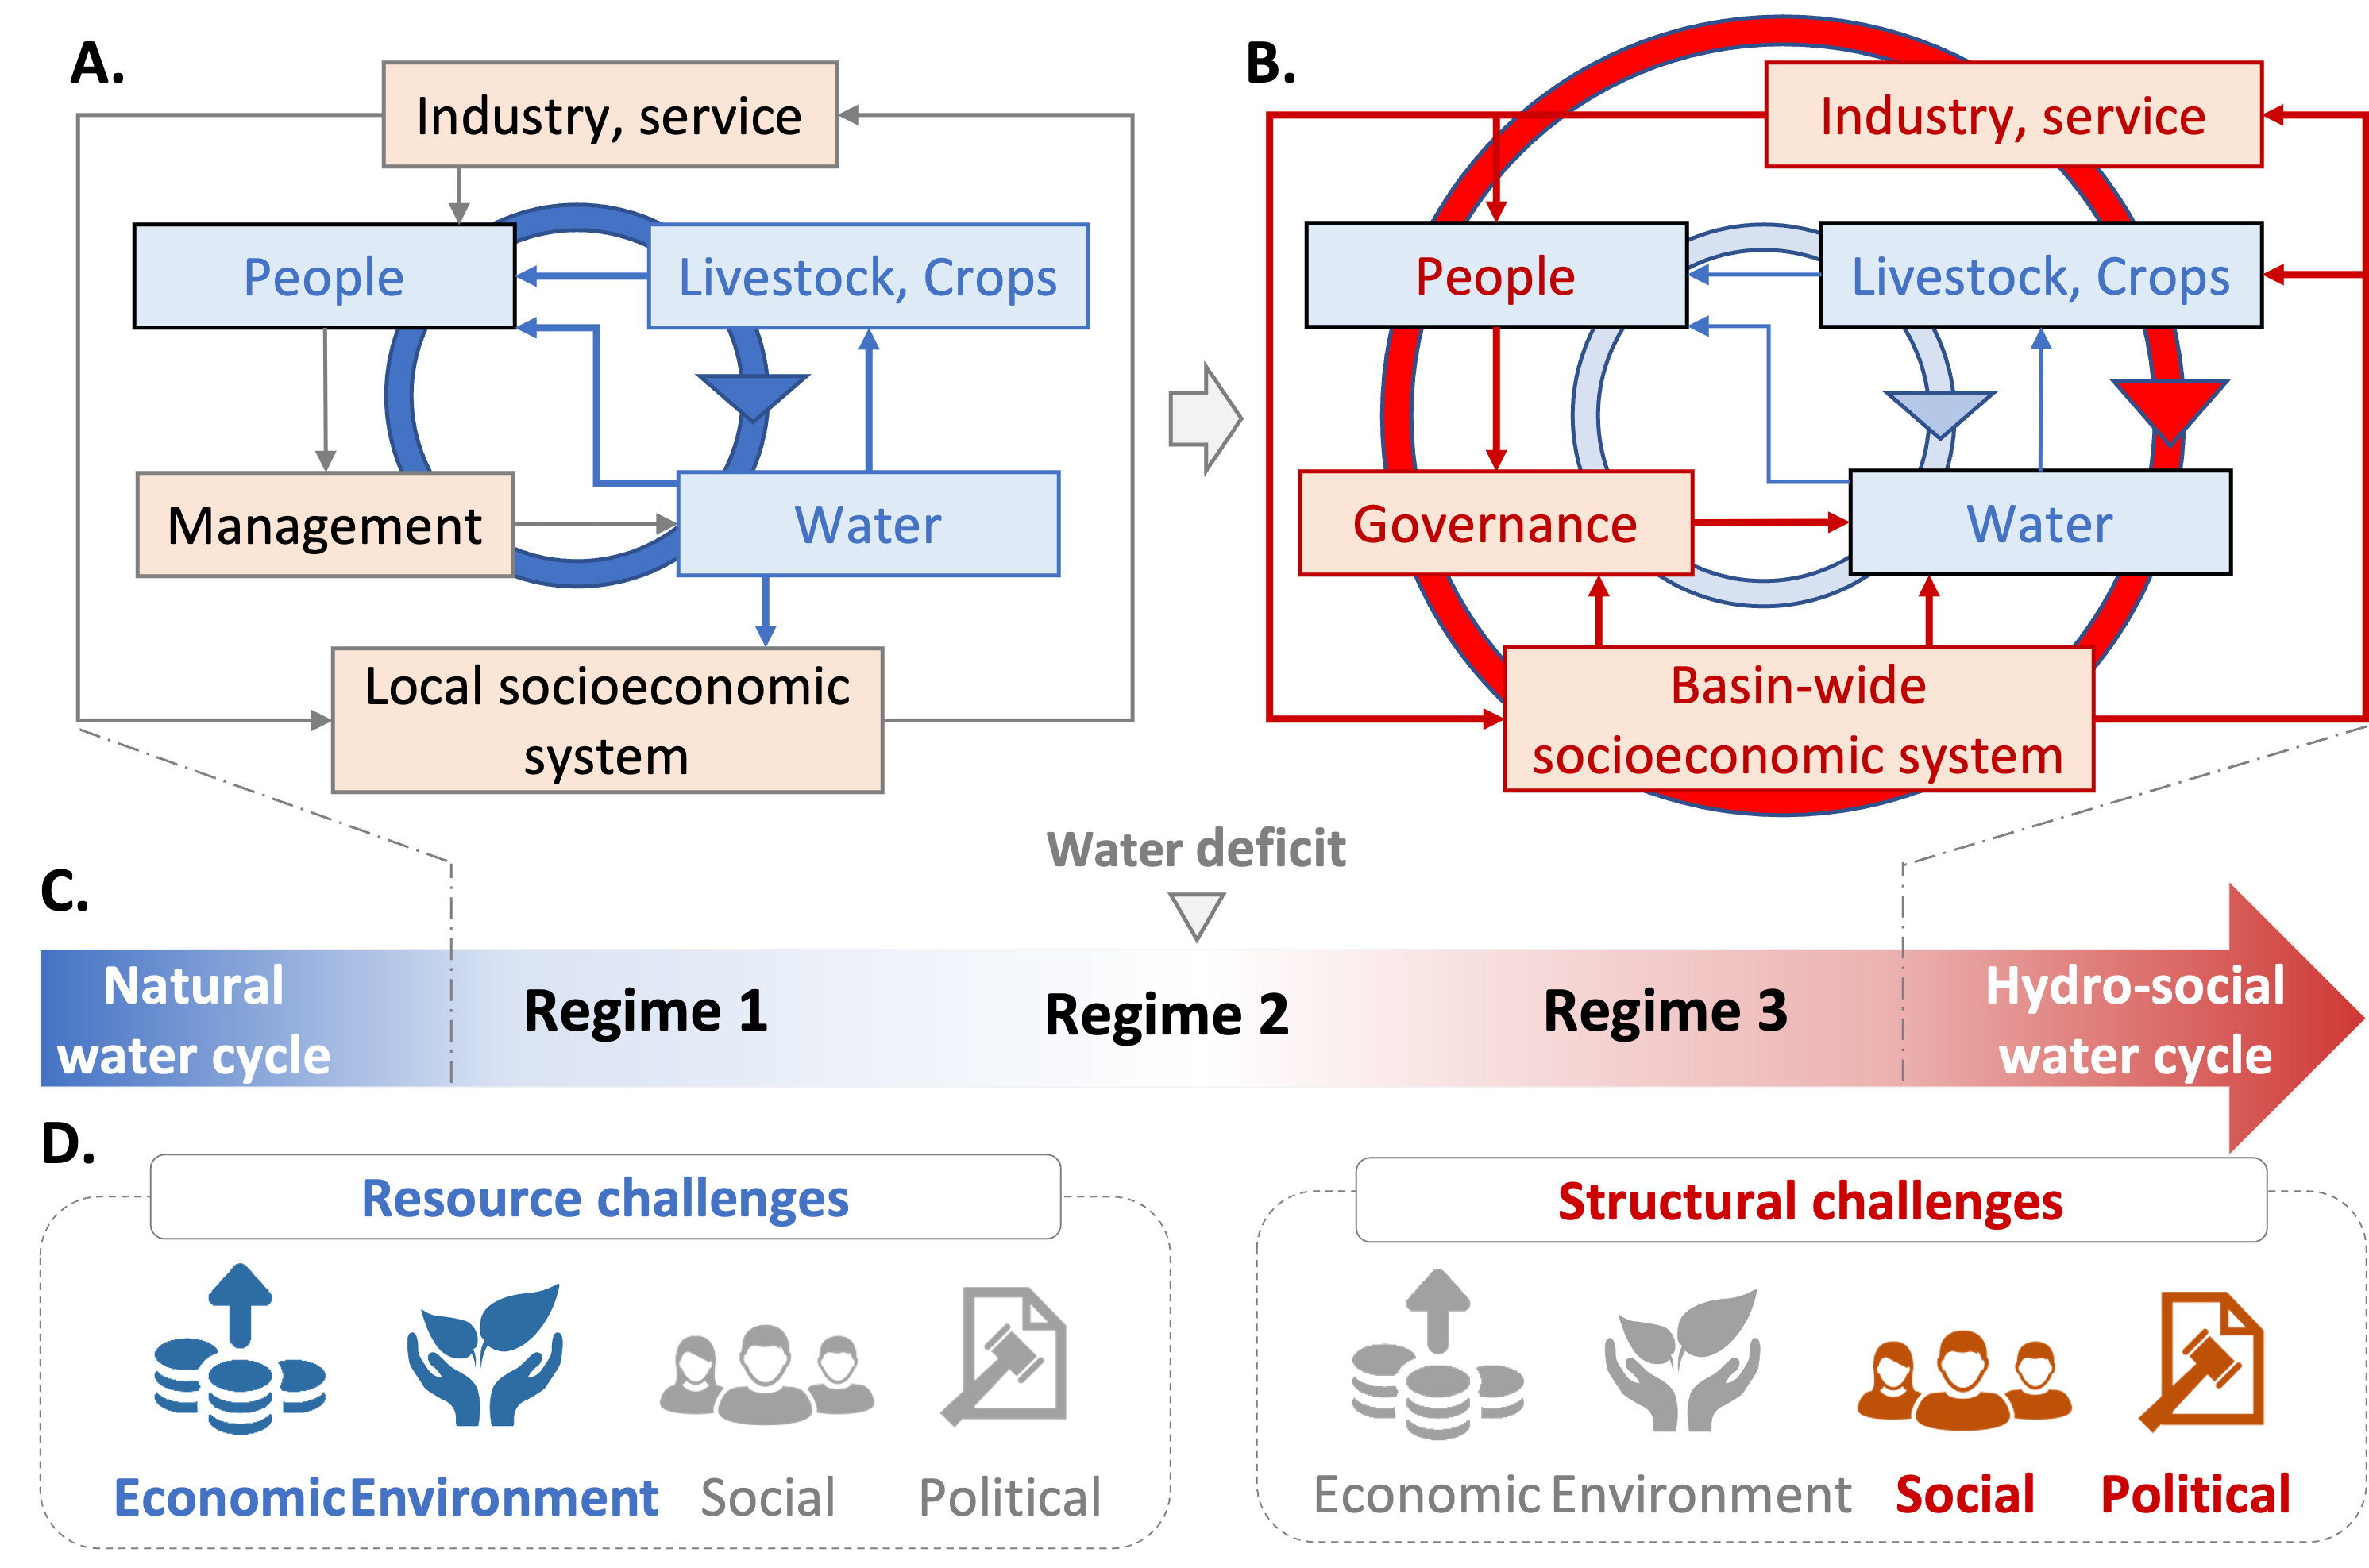
\includegraphics[width=0.8\linewidth]{main/transition.png}
	\caption{
		Transition schema in hydrosocial cycle and water governance regimes. The natural water cycle dominates blue pathways, while socio-economic feedback dominates red.
		The large circular arrows indicate the social and hydrological processes that dominate in different stages.
		Provisioning water includes water used by human, livestock and crops while non-provisioning water includes used by industry and service.
		The processes expressed in the graph mainly include: Water supports people in provisioning ways or influence/influenced socioeconomic systems as non-provisioning ways; People manage/govern water system based on their well-beings.
		The gray thick arrow represents weaker process, while the red arrow represents more significant one.
		\textbf{A.} As socio-economic systems develop, non-provisioning water demand increases; simultaneously, increased adaptive capacity by engineering allows people to manage water resources to alleviate water stress.
		\textbf{B.} With further growing socio-economic systems, trade-offs between provisioning-purpose and non-provisioning water use become prominent; a basin-wide socio-economic system requires more organized water governance.
		Thus, \textbf{C. the hydrosocial water cycle transition} correlates with the water governance regime shifts. The transformation governance regime shift occurs following the water deficit, with the rapid growth of adaptive capacity.
		\textbf{D. Water governance challenges} Through the transitional regimes, water governance faces primarily economic and environmental challenges but social and policy challenges later.
	}\label{fig:summary}
\end{figure*}


%* limitations & direction
One of the main limitations in the approach is the lack of multi-sources data in long-term period worldwide, which means there is still a gap between comprehensively identifying and applying the IWGI widely.
We propose that all water governance issues, however, can change ``who gets water, when and how'' so monitoring such an integrated index is essential, even use simpler indicators.
We suggest that choices of indicators for different aspects can be adopted according to available datasets -e.g., replace the SFV-index (IA) with simpler scarcity index or proportion-based purpose indicator (IP) by complicated one.
Another limitation is the lack of latest datasets which is coherent with the historical datasets, so our analysis had to discontinued in 2013 despite potential shifts existing.
As a supplement, we examined IWGI framework with fewer datasets from different source in recent decades where showing no significant regime changes (supplementary Figure~\ref{fig:summary}).  % TODO 补充材料新图
Therefore, we suggest IWGI framework can be applied with adaptive indicators and flexible time series according to accessible datasets in future studies.

In today's world, regime shifts from natural to human-dominated seem likely to become increasingly widespread; comprehensive strategies to address governance challenges will have to become the core of complex human-water systems~\cite{cumming2018,cumming2014,jaeger2019}.
Although river basins have shown improvements in water management technologies and water use efficiency, many are still approaching local, regional, and planetary boundaries where human-water systems may collapse~\cite{gleeson2020, wang-erlandsson2022}.
A deeper understanding of governance that incorporates ideas of non-linear regime shifts and transformations should help shift the focus of governance towards maintaining the resilience of the basin’s social-ecological system and improving its sustainability~\cite{falkenmark2019}.
